
\section{The Analysis}

Throughout the analysis, we assume that the expected approximation ratio of \rnk{} is at most $1/2 + c$ for some rational $c \geq 0$. Then, we prove that if $c$ is smaller than some constant, it leads to a contradiction. This implies a lower bound on the expected approximation ratio of \rnk{}. Moreover, we assume that, without loss of generality, $cn/2$ is an integer. To understand this, consider a graph where the approximation ratio of \rnk{} is $1/2 + c$ and $cn/2$ is not an integer. For $c=a/b$ with integers $a,b$, by copying the same graph $2b$ times, the approximation guarantee of \rnk{} remains unchanged, but now $cn'/2$ is an integer, where $n'=2bn$ is the number of vertices in the new graph. Our proof relies on counting a structure in the graph, referred to as a $k$-wasteful independent set ($k$-\wis), which we define formally in \Cref{def:ltap}. 
Next, in \Cref{lem:kltap-all-perms}, we demonstrate a lower bound on the expected number of $k$-WIS if the approximation ratio of \rnk{} is at most $1/2 + c$. Further, in \Cref{lem:upperbound-kwis}, we prove an upper bound on the number of $k$-WIS. Finally, in \Cref{thm:final}, we combine these bounds to show a lower bound for the constant $c$.


\begin{definition}[$k$-wasteful independent set ($k$-\wis)]\label{def:ltap}
Given matching $R$ the output of \rnk{}, a subset of $2k$ vertices $I$ is a $k$-wasteful independent set, iff vertices in $I$ are end-points of $k$ length-three augmenting paths in $R\oplus \opt{}$. This also implies that $I$ is an independent set of $G$ since \rnk{} outputs a maximal matching and vertices in $I$ are left unmatched in $R$. Figure~\ref{figure:8934} shows an example of a 5-\wis{}.
\end{definition}

\usetikzlibrary{decorations.pathmorphing}

\begin{figure}[h!]
    \centering
    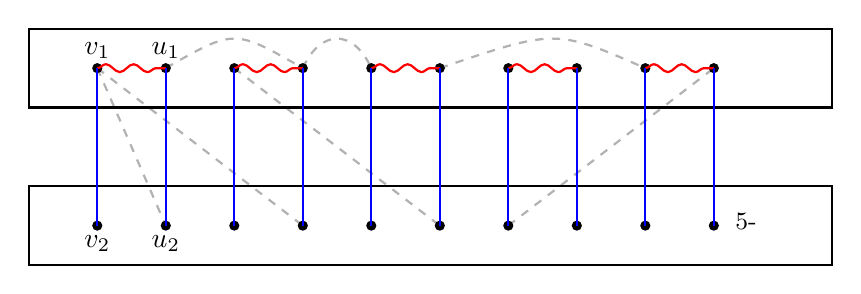
\begin{tikzpicture}[scale=0.5]     % Adjust the scale factor here
        % Scale factor for wider picture
        \pgfmathsetmacro{\scaleFactor}{1.2}

        % Define a lighter gray color
        \definecolor{lightergray}{gray}{0.7}

        % Draw a half-oval lighter gray dashed edge between vertex 2 and vertex 4 inside the rectangle
        \draw[lightergray, thick, dashed] (2.9 * \scaleFactor, 1) .. controls (4.35 * \scaleFactor, 2) and (4.35 * \scaleFactor, 2) .. (5.8 * \scaleFactor, 1);

        % Draw a half-oval lighter gray dashed edge between vertex 4 and vertex 5 inside the rectangle
        \draw[lightergray, thick, dashed] (5.8 * \scaleFactor, 1) .. controls (6.175 * \scaleFactor, 2) and (6.875 * \scaleFactor, 2) .. (7.25 * \scaleFactor, 1);

        % Draw a half-oval lighter gray dashed edge between vertex 6 and vertex 10 inside the rectangle
        \draw[lightergray, thick, dashed] (8.7 * \scaleFactor, 1) .. controls (11.15 * \scaleFactor, 2) and (11.15 * \scaleFactor, 2) .. (13.05 * \scaleFactor, 1);

        % Draw a straight lighter gray dashed edge between the first vertex in the top rectangle and the second vertex from the bottom
        \draw[lightergray, thick, dashed] ({1.45 * \scaleFactor}, 1) -- ({2.9 * \scaleFactor}, -3);

        % Draw a straight lighter gray dashed edge between the first vertex in the top rectangle and the fourth vertex from the bottom
        \draw[lightergray, thick, dashed] ({1.45 * \scaleFactor}, 1) -- ({5.8 * \scaleFactor}, -3);

        % Draw a straight lighter gray dashed edge between the 7th vertex from the bottom and the 10th vertex from the top
        \draw[lightergray, thick, dashed] ({10.15 * \scaleFactor}, -3) -- ({14.5 * \scaleFactor}, 1);

        % Draw a straight lighter gray dashed edge between the third vertex from the top and the sixth vertex from the bottom
        \draw[lightergray, thick, dashed] ({4.35 * \scaleFactor}, 1) -- ({8.7 * \scaleFactor}, -3);

        % Draw the first horizontal rectangle (20% wider)
        \draw[thick] (0,0) rectangle (17 * \scaleFactor, 2);

        % Draw the 10 vertices inside the first rectangle, sorted on a horizontal line, avoiding borders
        \foreach \i in {1,...,10} {
            \node[circle, fill, inner sep=1.3pt] at ({1.45 * \scaleFactor + 1.45 * \scaleFactor * (\i-1)}, 1) {};
        }

        % Add names to the first two vertices from the top
        \node[anchor=south] at ({1.45 * \scaleFactor}, 1) {\(v_1\)};
        \node[anchor=south] at ({2.9 * \scaleFactor}, 1) {\(u_1\)};

        % Add label inside the upper rectangle on the right side after all the vertices
        % \node[anchor=west] at ({17 * \scaleFactor - 2}, 1) {$R$};

        % Draw the five matching edges between vertices in the top rectangle (red and wiggly)
        \foreach \i in {0,2,4,6,8} {
            \draw[red, thick, decorate, decoration={snake, amplitude=0.5mm}] ({1.45 * \scaleFactor + 1.45 * \scaleFactor * \i}, 1) -- ({1.45 * \scaleFactor + 1.45 * \scaleFactor * (\i+1)}, 1);
        }

        % Draw the second horizontal rectangle (20% wider)
        \draw[thick] (0,-4) rectangle (17 * \scaleFactor, -2);

        % Draw the 10 vertices inside the second rectangle, sorted on a horizontal line, avoiding borders
        \foreach \i in {1,...,10} {
            \node[circle, fill, inner sep=1.3pt] at ({1.45 * \scaleFactor + 1.45 * \scaleFactor * (\i-1)}, -3) {};
        }

        % Add names to the first two vertices from the bottom
        \node[anchor=north] at ({1.45 * \scaleFactor}, -3) {\(v_2\)};
        \node[anchor=north] at ({2.9 * \scaleFactor}, -3) {\(u_2\)};

        % Add label inside the lower rectangle on the right side after all the vertices
        \node[anchor=west] at ({17 * \scaleFactor - 2.7}, -2.9) {\small{5-\wis{}}};

        % Draw blue edges from each vertex in the top rectangle to the corresponding vertex in the bottom rectangle
        \foreach \i in {1,...,10} {
            \draw[blue, thick] ({1.45 * \scaleFactor + 1.45 * \scaleFactor * (\i-1)}, 1) -- ({1.45 * \scaleFactor + 1.45 * \scaleFactor * (\i-1)}, -3);
        }

    \end{tikzpicture}
   \caption{\small{The red edges are from matching $R$ outputted by \rnk{} and the blue ones are from \opt{}. The lower vertices form a 5-\wis{} as they are the endpoints of five length-three augmenting.}}
    \label{figure:8934}
\end{figure}



\begin{lemma}[Lower Bound on the Expected Number of $k$-\wis{}]\label{lem:kltap-all-perms}
    If the approximation ratio of \rnk{} is at most $1/2 + c$ for $0 \leq c \leq 1/6$, then the expected number of $k$-WIS in the output of \rnk{} is at least one, when $k = (1/2 - 3c) \cdot n/2$.
\end{lemma}
\begin{proof}
    First, if the size of the matching produced by \rnk{} for some permutation is $(1/2 + c) \cdot n/2$, then there exist at least $(1/2 - 3c)\cdot n/2$ disjoint length-three augmenting paths by \Cref{prop:aug3-path-bound}. Let $\mu_1, \ldots, \mu_{n!}$ be the sizes of the matchings produced by \rnk{} for all different permutations such that $\mu_i = (1/2 + c_i)\cdot n/2$ for some $c_i \geq 0$ (such $c_i$ always exists since the output of \rnk{} is a maximal matching). For the $i$th permutation, there exist at least $(1/2 - 3c_i)\cdot n/2$ length-three augmenting paths. Therefore, the total number of length-three augmenting paths in all permutations, denoted by $s$, is at least
    \begin{align*}
        s = \sum_{i=1}^{n!} (\frac{1}{2} - 3c_i)\cdot \frac{n}{2} = \frac{n \cdot n!}{4} - \frac{3n}{2} \sum_{i=1}^{n!} c_i   \geq
        (n!) \cdot \left( \frac{n}{4} - \frac{3nc}{2}\right),
    \end{align*}
    where the last inequality is followed by the fact that the approximation ratio of the algorithm is at least $1/2 + c$. Let $a_i$ be the number of length-three augmenting paths in the $i$th permutation. There exist at least ${ a_i \choose k}$ number of $k$-WIS in the $i$th permutation. It follows that the total number of $k$-WIS is $\sum_{i=1}^{n!} {a_i \choose k}$. Moreover, $\sum_{i=1}^{n!} {a_i \choose k}$ is minimized when all $a_i$'s are equal due to \Cref{prop:bionomila-minimize}. Therefore, the total number of $k$-WIS is at least
    \begin{align*}
        \sum_{i=1}^{n!} {a_i \choose k} \geq n! \cdot {s/n! \choose k} = n! \cdot {n/4 - 3nc/2 \choose n/4 - 3nc/2} = n!,
    \end{align*}
    which implies that the expected number of $k$-WIS is at least one.
\end{proof}



\begin{claim}\label{clm:kltap-bound}
    There exist at most ${n/2 \choose 2k} \cdot 3^k$ \underline{different} $k$-WIS for all possible outputs of \rnk{} on input graph $G$.
\end{claim}
\begin{proof}
    First, we select $2k$ edges from \opt{} that will create $k$ length-three augmenting paths in \Cref{def:ltap}. This selection has ${n/2 \choose 2k}$ possible combinations. To determine which endpoints of these edges will form $I$ (the $k-$\wis{}) in \Cref{def:ltap}, there are $2^{2k}$ possible choices. We further show that this is at most $3^k$. Consider the collection of $k$ length-three alternating paths denoted by $L$. Suppose there is an augmenting path $(v_2, v_1, u_1, u_2)$ in $L$ (for instance, see \Cref{figure:8934}). In this case, we can rule out the possibility of both $v_1$ and $u_1$ being present in $I$ simultaneously, since there is an edge between $v_1$ and $u_1$, and $I$ must be an independent set. Now apply this process to all $k$ augmenting paths in $L$. For each pair of edges in \opt{} that appear in the same length-three augmenting path in $L$, there are 3 possible choices for which endpoint can be included in $I$, since the endpoints of the middle edge in the augmenting path cannot both be in $I$. Consequently, the total number of different possible $k$-WIS is at most ${n/2 \choose 2k} \cdot 3^k$.
\end{proof}






\begin{claim}\label{lem:prob-bound}
Let $I = \{v_1, v_2, \ldots, v_{2k}\}$ be a set of independent vertices in $G$. Then, the vertices in $I$ form a $k$-WIS with probability at most $1/2^{2k}$ in the output of \rnk{}.
\end{claim}

\begin{proof}
Let $E_I$ denote the set of edges in \opt{} that have at least one endpoint in $I$. Since \opt{} is a perfect matching and $I$ is an independent set, we have $|E_I| = 2k$, and $E_I$ covers all vertices in $I$. Let $V(E_I)$ be the set of endpoints of $E_I$ and $\bar{I} = V(E_I) \setminus I$. For the edges in $E_I$ to form length-three augmenting paths, they must be partitioned into pairs, with each pair creating one length-three augmenting path.


Let \((v_1, v_2)\) and \((u_1, u_2)\) be such a pair with \(v_2\) and \(u_2\) in \(I\) (for instance, see \Cref{figure:8934}). Then there must exist an edge between \(v_1\) and \(u_1\) to form the augmenting path. We claim that \(\pi(v_1) < \pi(u_2)\) if $\pi$ is the permutation chosen by \rnk{}. To prove this by contradiction, assume that $\pi(v_1) > \pi(u_2)$. When $u_2$ is processed by \rnk{}, since it is wasted (unmatched in $R$), it must be available and have no free neighbor. In particular, this means $u_1$ is matched and has a match with rank less than $\pi(u_2)$. However, this implies that $\pi(\text{match of } u_1) < \pi(u_2) < \pi(v_1)$, contradicting the fact that $u_1$ is matched with $v_1$ in $R$. Thus, we have \(\pi(v_1) < \pi(u_2)\). We call $u_2$ in this case the {\em counterpart} of $v_1$ and let $C(v_1)$ denote the counterpart of $v_1$. For each vertex in $\bar{I}$, its counterpart is a unique vertex in $I$. Hence, the set of all counterparts of vertices in $\bar{I}$ is $I$. Using the same argument, we can show that for all vertices $v\in \bar{I}, \pi(v)< \pi(C(v))$.


If we consider a permutation of the vertices in $I \cup \bar{I}$, it must satisfy the property described in the above argument for $I$ to be a $k$-\wis{}. In the remainder of the proof, we will focus on calculating the probability of this property being satisfied. Let $\sigma$ be a permutation over vertices in $\bar{I}$. In each iteration, we add a new vertex from $I$ to the permutation such that it does not violate the property. Let $u$ be the last vertex in \(\sigma\). In the permutation of vertices in \(I\) and \(\bar{I}\), \(C(u)\) can appear only after \(u\), and since \(u\) is the last element in \(\bar{I}\), the relative place of \(C(u)\) with respect to \(\sigma\) is only after its last element. For \(C(u)\) to be after all elements in \(\sigma\), which has length \(2k\), it has a probability of \(1/(2k+1)\) since the permutation that \rnk{} chooses is uniformly at random. 


Let $u_i$ be the $i$th vertex from the end in $\sigma$. When we add the counterpart of $u_i$, there are $2i - 1$ positions (from the end of the permutation to the one right after $u_i$\footnote{As the counterparts of the last $i-1$ vertices are all placed after $u_i$, there are, in total, $2(i-1)+1=2i-1$ slots where we can put $C(u_i)$ to make $\pi(u_i)<\pi(C(u_i))$ hold.}) among the available $(2k + i)$ positions where we can place it. Therefore, 
\begin{align*}
    \Pr[\text{ $I$ is a $k$-WIS in output of \rnk{} }] \leq& \prod_{i=1}^{2k} \frac{2i - 1}{2k+i}\\
     =& \frac{(4k)! / (\prod_{i=1}^{2k} 2i)}{\prod_{i=1}^{2k} (2k + i)}\\
     =& \frac{(4k)! / ((2k)! \cdot 2^{2k})}{(4k)!/(2k)!} = \frac{1}{2^{2k}}.
\end{align*}
\end{proof}




\begin{lemma}[Upper Bound on the Expected Number of $k$-\wis{}]\label{lem:upperbound-kwis}
    The expected number of $k$-\wis{} in the output of \rnk{} is at most ${n/2 \choose 2k} \cdot (3/4)^k$.
\end{lemma}

\begin{proof}
    By \Cref{clm:kltap-bound}, there exist at most ${n/2 \choose 2k} \cdot 3^k$ different $k$-\wis{}. Also, each of them has a probability $1/(2^{2k})$ to be in the output of \rnk{} by \Cref{lem:prob-bound}. Thus, by the linearity of the expectation, the expected number of $k$-\wis{} in the output of \rnk{} is at most ${n/2 \choose 2k} \cdot (3/4)^k$.
\end{proof}


\begin{theorem}\label{thm:final}
The expected approximation ratio of \rnk{} is at least $0.505$ in general graphs.
\end{theorem}

\begin{proof}
    Suppose that the approximation ratio of \rnk{} is at most $1/2 + c$ for $c \leq 0.005$. Let $k = (1/2 - 3c)\cdot n/2$. By \Cref{lem:kltap-all-perms}, the expected number of $k$-\wis{} is at least one. On the other hand, by \Cref{lem:upperbound-kwis}, the expected number of $k$-\wis{} is at most ${n/2 \choose 2k} \cdot (3/4)^k$. Hence, it must hold that ${n/2 \choose 2k} \cdot (3/4)^k \geq 1$. Now, we show that this cannot happen for $c\leq 0.005$. In particular, we have
        \begin{align*}
        &{n/2 \choose 2k} \cdot \left(\frac{3}{4}\right)^k\\
         =& {n/2 \choose (1-6c) \cdot n/2} \cdot \left(\frac{3}{4}\right)^{(1/2 - 3c)\cdot n/2} & (\text{Since } k = (1/2 - 3c)\cdot n/2)\\
        =&{n/2 \choose 6c \cdot n/2} \cdot \left(\frac{3}{4}\right)^{(1/2 - 3c)\cdot n/2} & (\text{By the identity of binomial coefficients})\\
        \leq& 2^{(n/2) \cdot H(6c)} \cdot \left(\frac{3}{4}\right)^{(1/2 - 3c)\cdot n/2} & (\text{By \Cref{prop:entropy-approximation}})\\
        =&2^{(n/2)\cdot H(6c)}\cdot 2^{(n/2)\cdot \log_2(\frac{3}{4})\cdot(1/2 - 3c)}\\
        =&2^{(n/2)\cdot [H(6c)+\log_2(\frac{3}{4})\cdot(1/2 - 3c)]}\\
        <& 1 &(\text{When $c\leq 0.005,\;H(6c)+\log_2(\frac{3}{4})\cdot(1/2 - 3c)<0$}),
    \end{align*}
    which is a contradiction. Therefore, $c$ cannot be smaller than $0.005$ as otherwise, we obtain ${n/2 \choose 2k} \cdot (3/4)^k < 1$ which completes the proof.
\end{proof}